\documentclass[12pt]{beamer}

\usepackage{beamerthemeHannover, graphicx, clrscode, amsmath, amssymb, multicol}
\setbeamercolor{sidebar}{use=structure,bg=gray!20!green!60!white}

\title{Scientific Computing With Perl and Math::GSL}
\author[J.A. Leto]{Jonathan Leto\\jonathan@leto.net}
\date{}

\begin{document}
\frame{
    \titlepage
    \begin{center}
    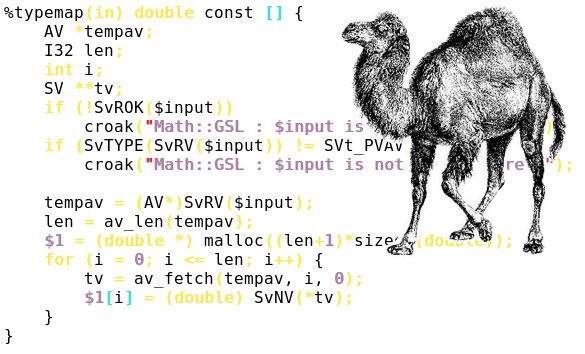
\includegraphics[width=5.84cm, height=3.85cm]{swig_camel}
    \end{center}
}

\section{Philosophy}
\frame{
    \frametitle{Don't Write Glue}
    \begin{center}
    \begin{columns}[t]
        \begin{column}{5cm}
          %  
\includegraphics[width=5.00cm, height=5.00cm]{xs_is_glue}
        \end{column}
        \begin{column}{5cm}
          %  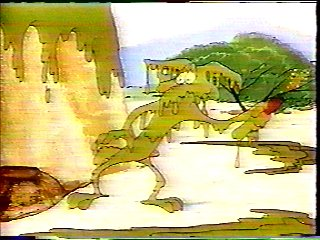
\includegraphics[width=5.00cm, height=5.00cm]{acmeglue}
        \end{column}
    \end{columns}
    \end{center}

}

\section{Going Forward}

\frame{
    \frametitle{Active Development Continues}

    \begin{itemize}
        \item Scientific Computing applications built on top of Math::GSL
        \item Full gsl\_function callback support
        \item Static libraries and error handlers
        \item Porting to Darwin and Solaris
        \item Threads
    \end{itemize}
}
\section{Acknowledgements}
\frame{
    \frametitle{Thanks}

    \begin{itemize}
        \item Device::Cdio
        \item Thierry Moisan
        \item Eric Wilhelm
        \item \#pdx.pm
        \item Leslie Hawthorn
        \item The entire Google Summer of Code crew
    \end{itemize}
}

\frame{
    \frametitle{More Info}
    \begin{itemize}
        \item {http://www.swig.org}\\
        \item {http://leto.net/gitweb/}\\
        \item {http://leto.net/code/Math-GSL/}\\
        \item {http://groups.google.com/group/math-gsl-dev}\\
        \item {http://groups.google.com/group/perl-scientific-computing}\\
    \end{itemize}

}

\end{document}
